% =================================================================
%  JURNAL ILMU KOMPUTER DAN AGRI-INFORMATIKA (JIKA)
%  Implementasi Protokol AAA, Enkripsi Kolom, dan Tanda Tangan
%  Digital pada Aplikasi TUMBUH
%
%  KOM1315 Keamanan Informasi — Kelompok 9
%  Semester Genap 2025/2026, IPB University
%
%  Kompilasi: pdflatex -> bibtex -> pdflatex -> pdflatex
% =================================================================

\documentclass[12pt,a4paper]{article}

% ── Encoding & bahasa ─────────────────────────────────────────
\usepackage[T1]{fontenc}
\usepackage{textcomp}
\usepackage[utf8]{inputenc}
\usepackage[english]{babel}

% ── Font ──────────────────────────────────────────────────────
\usepackage{mathptmx}
\usepackage{microtype}

% ── Layout: JIKA — kiri 3cm, lainnya 2cm, spasi tunggal ──────
\usepackage[a4paper, top=2cm, bottom=2cm,
            left=3cm, right=2cm, headheight=14pt]{geometry}
\usepackage{setspace}
\singlespacing
\usepackage{indentfirst}
\setlength{\parindent}{1cm}
\setlength{\parskip}{3pt}

% ── Header/footer ─────────────────────────────────────────────
\usepackage{fancyhdr}
\pagestyle{fancy}
\fancyhf{}
\fancyhead[L]{\small\itshape Jurnal Ilmu Komputer dan Agri-informatika}
\fancyhead[R]{\small\thepage}
\renewcommand{\headrulewidth}{0.4pt}
\fancypagestyle{plain}{\fancyhf{}\fancyhead[R]{\small\thepage}%
  \renewcommand{\headrulewidth}{0pt}}

% ── Format judul bab/subbab (JIKA: 14pt/12pt, rata kiri) ─────
\usepackage{titlesec}
\titleformat{\section}
  {\normalfont\bfseries\fontsize{14pt}{16pt}\selectfont}
  {\thesection.}{0.5em}{}
\titlespacing*{\section}{0pt}{14pt}{6pt}
\titleformat{\subsection}
  {\normalfont\bfseries\fontsize{12pt}{14pt}\selectfont}
  {\thesubsection}{0.5em}{}
\titlespacing*{\subsection}{0pt}{10pt}{4pt}

% ── Tabel ─────────────────────────────────────────────────────
\usepackage{booktabs}
\usepackage{array}
\usepackage{tabularx}
\usepackage{multirow}
\usepackage{makecell}
\usepackage{float}

% ── Gambar ────────────────────────────────────────────────────
\usepackage{graphicx}
\graphicspath{{../draft_dari_laporan/latex/}}

% ── Caption: JIKA 9pt rata tengah ────────────────────────────
\usepackage{caption}
\captionsetup{font=small, labelfont={small,bf}, labelsep=period,
  justification=centering, singlelinecheck=true}
\captionsetup[figure]{name=Gambar, position=below, skip=4pt}
\captionsetup[table]{name=Tabel, position=above, skip=2pt}

% ── Listing kode ──────────────────────────────────────────────
\usepackage{listings}
\usepackage{xcolor}
\renewcommand{\lstlistingname}{Kode}
\definecolor{codegray}{gray}{0.95}
\definecolor{codecomment}{rgb}{0.38,0.44,0.50}
\definecolor{codekw}{rgb}{0.10,0.20,0.55}
\definecolor{codestr}{rgb}{0.55,0.10,0.10}
\lstset{
  basicstyle=\ttfamily\footnotesize,
  backgroundcolor=\color{codegray},
  commentstyle=\color{codecomment}\itshape,
  keywordstyle=\color{codekw}\bfseries,
  stringstyle=\color{codestr},
  numbers=left, numberstyle=\ttfamily\scriptsize\color{codecomment},
  numbersep=8pt, frame=single, framesep=4pt,
  rulecolor=\color{gray!40}, breaklines=true,
  showstringspaces=false, tabsize=2, captionpos=b,
  columns=fullflexible, keepspaces=true,
  xleftmargin=14pt, aboveskip=6pt, belowskip=6pt,
  extendedchars=false
}

% ── Matematika ────────────────────────────────────────────────
\usepackage{amsmath,amssymb}

% ── Bibliografi (Harvard/IPB) ─────────────────────────────────
\usepackage[authoryear,round,sort&compress]{natbib}
\setcitestyle{aysep={}}
\setlength{\bibsep}{2pt}

% ── Hyperref ──────────────────────────────────────────────────
\usepackage[colorlinks=false, hidelinks]{hyperref}
\usepackage{url}
\usepackage{enumitem}

% =================================================================
\begin{document}
\pagestyle{fancy}
% =================================================================

% ── Blok judul (format JIKA) ──────────────────────────────────
\begin{flushleft}
{\fontsize{16pt}{20pt}\selectfont\bfseries
Implementasi Protokol AAA, Enkripsi Kolom, dan Tanda Tangan Digital
pada Aplikasi TUMBUH}\\[6pt]
{\fontsize{14pt}{17pt}\selectfont\itshape
Implementation of AAA Protocol, Column Encryption, and Digital
Signature in the TUMBUH Application}\\[10pt]
RAFIF MUHAMMAD FARRAS$^{1*}$,
ADAM NAUFAL$^{1}$,
GHIFFARI BRAVIA HISHAM$^{1}$
\end{flushleft}

\vspace{2pt}
\noindent\rule{\textwidth}{0.4pt}
\begin{flushleft}
{\fontsize{9pt}{11pt}\selectfont
$^{1}$Departemen Ilmu Komputer, Fakultas Matematika dan Ilmu
Pengetahuan Alam, IPB University, Bogor 16680\\
$^{*}$Penulis Korespondensi: Rafif Muhammad Farras;
Tel: 081284314322; Surel: rafiffarras23@gmail.com\\
Adam Naufal; Tel: 081293625601; Surel: adaman507@gmail.com\\
Ghiffari Bravia Hisham; Tel: 081286714480;
Surel: ghiffari.bravia.hisham@gmail.com}
\end{flushleft}
\noindent\rule{\textwidth}{0.4pt}

\vspace{8pt}

% ── Abstrak (Indonesia) ───────────────────────────────────────
\noindent\textbf{Abstrak.} TUMBUH merupakan aplikasi web pelacak
karier dan magang untuk komunitas akademik IPB University yang
mengelola data sensitif mahasiswa, meliputi identitas, dokumen CV,
surat lamaran, dan status seleksi. Meningkatnya ancaman siber dan
berlakunya Undang-Undang Pelindungan Data Pribadi No.\,27 Tahun 2022
mendorong penerapan kontrol keamanan terstruktur pada sistem semacam
ini. Penelitian ini merancang dan mengimplementasikan kerangka
keamanan berlapis pada TUMBUH berdasarkan protokol autentikasi,
otorisasi, dan akuntansi yang diperkuat enkripsi simetris dan tanda
tangan digital. Autentikasi menggunakan hashing kata sandi bcrypt,
token berbasis JSON Web Token algoritma HS256, dan Google OAuth.
Otorisasi menerapkan kendali akses berbasis peran dengan pemeriksaan
kepemilikan data. Akuntansi dilakukan oleh mikroservis audit terpisah
yang menjaga integritas catatan melalui rantai hash SHA-256. Enkripsi
tingkat kolom Fernet melindungi kerahasiaan surat lamaran dari
kebocoran basis data, sedangkan tanda tangan digital Ed25519
memberikan jaminan non-repudiasi pada peristiwa lamaran. Seluruh modul
kriptografi terintegrasi langsung dalam alur utama aplikasi, bukan
sebagai skrip terpisah, dan semua kunci dikelola melalui variabel
lingkungan. Pengujian unit pada sembilan skenario, mencakup
\textit{roundtrip} enkripsi-dekripsi, deteksi pemalsuan tanda tangan,
penolakan akses, dan penolakan \textit{ciphertext} yang rusak,
menghasilkan sembilan kelulusan. Hasil ini membuktikan kontrol yang
diimplementasikan memenuhi sasaran kerahasiaan, integritas, dan
akuntabilitas dalam cakupan yang diuji. Benchmark tambahan menunjukkan
bahwa overhead terbesar berada pada jalur login karena verifikasi
bcrypt, yaitu 276,4189 ms dibanding baseline sintetis 0,0002 ms,
sedangkan overhead submit dan read tetap kecil, masing-masing 0,1224
ms dan 0,0625 ms. Enkripsi surat lamaran berukuran 1007 byte
menghasilkan data tersimpan 1427 byte atau overhead 1,42x.

\vspace{4pt}
\noindent\textbf{Kata kunci.} autentikasi, enkripsi kolom, keamanan
informasi, kendali akses berbasis peran, non-repudiasi, tanda tangan
digital

\vspace{6pt}

% ── Abstract (English) ────────────────────────────────────────
\noindent\textbf{Abstract.} TUMBUH is a career and internship tracking
web application for the IPB University academic community. It handles
sensitive data, including student identities, CVs, application letters,
and selection statuses. Indonesia's Personal Data Protection Law
(Law No.\,27/2022) makes structured security controls a requirement
for systems that process such data. This paper documents the design and
implementation of a multi-layer security framework for TUMBUH based on
the AAA (Authentication, Authorization, Accounting) protocol, supported
by symmetric encryption and digital signatures. Authentication uses
bcrypt password hashing with automatic salting, JWT HS256 token
management (60-minute access tokens, 7-day refresh cycles), and Google
OAuth integration. Authorization uses a role-based access control
(RBAC) model across three roles with ownership verification. A separate
audit microservice handles accounting and protects log integrity through
SHA-256 hash chaining. Column-level Fernet encryption (AES-128-CBC +
HMAC-SHA256) keeps application letters confidential, and Ed25519
digital signatures provide non-repudiation on application events. All
cryptographic modules are integrated into the main application workflow
rather than run as standalone scripts, and all keys are stored in
environment variables with no hardcoded secrets. Unit testing covered
nine scenarios: encryption-decryption roundtrips, signature forgery
detection, access denial (HTTP 403), and corrupted ciphertext
rejection. All nine passed, confirming that the controls meet the
confidentiality, integrity, and accountability objectives within the
tested scope. A supplementary benchmark showed that the largest
overhead occurs in the login path because of bcrypt verification:
276.4189 ms compared with a synthetic baseline of 0.0002 ms. Submit
and read overhead remained small at 0.1224 ms and 0.0625 ms,
respectively. Encrypting a 1007-byte application letter produced a
1427-byte stored value, or a 1.42x storage overhead.

\vspace{4pt}
\noindent\textbf{Keywords.} authentication, column-level encryption,
digital signature, information security, non-repudiation, role-based
access control

\vspace{6pt}\noindent\rule{\textwidth}{0.4pt}\vspace{4pt}

% =================================================================
\section{PENDAHULUAN}
% =================================================================

Sistem informasi berbasis web yang mengelola proses rekrutmen dan
magang semakin umum di lingkungan perguruan tinggi. TUMBUH adalah
salah satunya, sebuah aplikasi yang menghubungkan mahasiswa IPB
University dengan perusahaan rekanan dan admin platform dalam satu
ekosistem daring. Mahasiswa dapat mencari lowongan, menyimpan daftar
favorit, dan mengirimkan lamaran; HR perusahaan mengelola lowongan dan
memantau proses seleksi; admin mengawasi keseluruhan sistem. Untuk
menjalankan fungsi-fungsi tersebut, sistem menyimpan data yang cukup
sensitif, yaitu identitas dan profil akademik mahasiswa, nomor induk
mahasiswa, dokumen CV, isi surat lamaran, hingga riwayat status seleksi
pelamar.

Karakteristik multi-peran sistem ini menghadirkan risiko keamanan yang
spesifik. Kata sandi yang lemah dan tidak adanya pembatasan percobaan
masuk membuka peluang tebak paksa (\textit{brute force}) dan
\textit{credential stuffing}. Jika otorisasi tidak diverifikasi di
setiap lapisan, data milik satu mahasiswa berpotensi diakses oleh
mahasiswa lain atau oleh HR dari perusahaan yang tidak relevan.
Kebocoran basis data pun tidak bisa diabaikan; surat lamaran yang
tersimpan sebagai teks biasa akan langsung terbaca jika berkas basis
data jatuh ke tangan yang salah. Yang lebih sulit ditangani adalah
risiko penyangkalan tindakan: mahasiswa yang menyangkal pernah
mengirimkan lamaran, atau perusahaan yang mengklaim tidak pernah
mengubah status seleksi. Tanpa catatan audit yang tahan gangguan dan
tanda tangan kriptografis pada setiap peristiwa, klaim semacam itu
sangat sulit dibantah \citep{Anderson2020}. Badan Siber dan Sandi
Negara melaporkan peningkatan insiden kebocoran data di sektor
pendidikan dalam beberapa tahun terakhir \citep{BSSN2023}, dan
berlakunya Undang-Undang Pelindungan Data Pribadi No.\,27 Tahun 2022
\citep{UUPDP2022} menjadikan penerapan kontrol keamanan bukan lagi
pilihan melainkan kewajiban hukum.

Keamanan informasi secara klasik diarahkan pada tiga sasaran utama,
yaitu kerahasiaan, integritas, dan ketersediaan data, yang pada sistem
multi-peran sering diperluas dengan akuntabilitas dan non-repudiasi
\citep{Stallings2017, Anderson2020}. Kerangka AAA, yang mencakup
\textit{Authentication}, \textit{Authorization}, dan
\textit{Accounting}, menyediakan struktur operasional untuk mencapai
sasaran-sasaran tersebut secara sistematis \citep{RFC2904}. Masing-masing
komponen kerangka ini telah diteliti cukup mendalam. Model kendali
akses berbasis peran dirumuskan oleh \citet{Sandhu1996} dan menjadi
standar otorisasi pada sistem multi-pengguna. Penyimpanan kata sandi
yang aman menggunakan bcrypt, sebuah fungsi hashing adaptif dengan
\textit{salt} otomatis yang secara eksplisit dirancang tahan terhadap
serangan tebak paksa \citep{Provos1999}. Untuk enkripsi data, standar
AES \citep{NIST2001} menjadi fondasi, dan spesifikasi Fernet
menggabungkan AES-128-CBC dengan HMAC-SHA256 untuk menghasilkan
enkripsi terautentikasi \citep{Katz2014, Cryptography2024}. Tanda
tangan digital Ed25519 berbasis Curve25519 dipilih atas dasar
keunggulan kinerja, ukuran tanda tangan yang ringkas, dan sifat
deterministiknya dibanding ECDSA \citep{Bernstein2012, RFC8032}.
Autentikasi berbasis token memanfaatkan JSON Web Token dengan algoritma
HS256 \citep{RFC7519} dan OAuth 2.0 untuk federasi identitas pihak
ketiga \citep{RFC6749}. Panduan identitas digital dari NIST
\citeyearpar{NISTSP80063B} memberikan acuan tentang siklus hidup token
yang aman, termasuk persyaratan masa berlaku dan mekanisme pencabutan.

Meskipun komponen-komponen tersebut sudah mapan secara individual,
dokumentasi implementasi yang mengintegrasikan seluruhnya dalam satu
alur kerja aplikasi web akademik masih jarang tersedia. Sebagian besar
implementasi yang terdokumentasi hanya mencakup satu atau dua aspek,
misalnya autentikasi berbasis token atau penerapan RBAC, tanpa
menyertakan enkripsi tingkat kolom pada atribut data tertentu maupun
tanda tangan digital per peristiwa bisnis. OWASP Top Ten
\citep{OWASP2021} menempatkan \textit{Broken Access Control} dan
\textit{Cryptographic Failures} sebagai dua kelemahan paling umum pada
aplikasi web, keduanya bersesuaian langsung dengan ancaman yang
dihadapi TUMBUH.

Penelitian ini bertujuan mengimplementasikan dan mendokumentasikan
kerangka keamanan berlapis pada TUMBUH yang mencakup protokol AAA
secara menyeluruh, enkripsi tingkat kolom berbasis Fernet, tanda tangan
digital Ed25519 untuk non-repudiasi, dan rantai hash SHA-256 untuk
integritas catatan audit. Seluruh komponen terintegrasi dalam alur
kerja utama aplikasi dan diverifikasi melalui pengujian unit.

% =================================================================
\section{METODE}
% =================================================================

Penelitian ini menggunakan pendekatan studi kasus berbasis implementasi
dalam konteks perkuliahan \textit{Problem-Based Learning} (PBL) mata
kuliah Keamanan Informasi (KOM1315) IPB University, Semester Genap
2025/2026.

\subsection{Desain Penelitian}

Pelaksanaan proyek mengikuti siklus berurutan: identifikasi aset dan
pemodelan ancaman, perancangan kontrol keamanan, implementasi kode,
integrasi ke alur kerja utama, dan pengujian unit. Tahap integrasi
secara khusus mensyaratkan bahwa seluruh modul kriptografi menyatu
dengan alur bisnis utama aplikasi, bukan dijalankan sebagai skrip
terpisah yang dapat dilewati.

\subsection{Deskripsi Sistem dan Arsitektur}

TUMBUH menggunakan arsitektur tiga komponen. \textit{Frontend}
dibangun dengan React dan Vite, berkomunikasi dengan \textit{backend}
melalui antarmuka REST \citep{Fielding2000}. \textit{Backend}
menggunakan FastAPI berbasis Python dengan ORM SQLAlchemy, yang
menyediakan validasi masukan otomatis melalui skema Pydantic dan
\textit{dependency injection} terstruktur untuk penerapan kontrol
otorisasi. Layanan audit berjalan sebagai mikroservis Node.js Express
yang terpisah. PostgreSQL melayani kebutuhan basis data, dan
komunikasi produksi dilindungi TLS 1.3 \citep{RFC8446}.
Gambar~\ref{fig:arsitektur} menunjukkan aliran data antarkomponen
beserta penempatan kontrol kriptografi.

\begin{figure}[H]
  \centering
  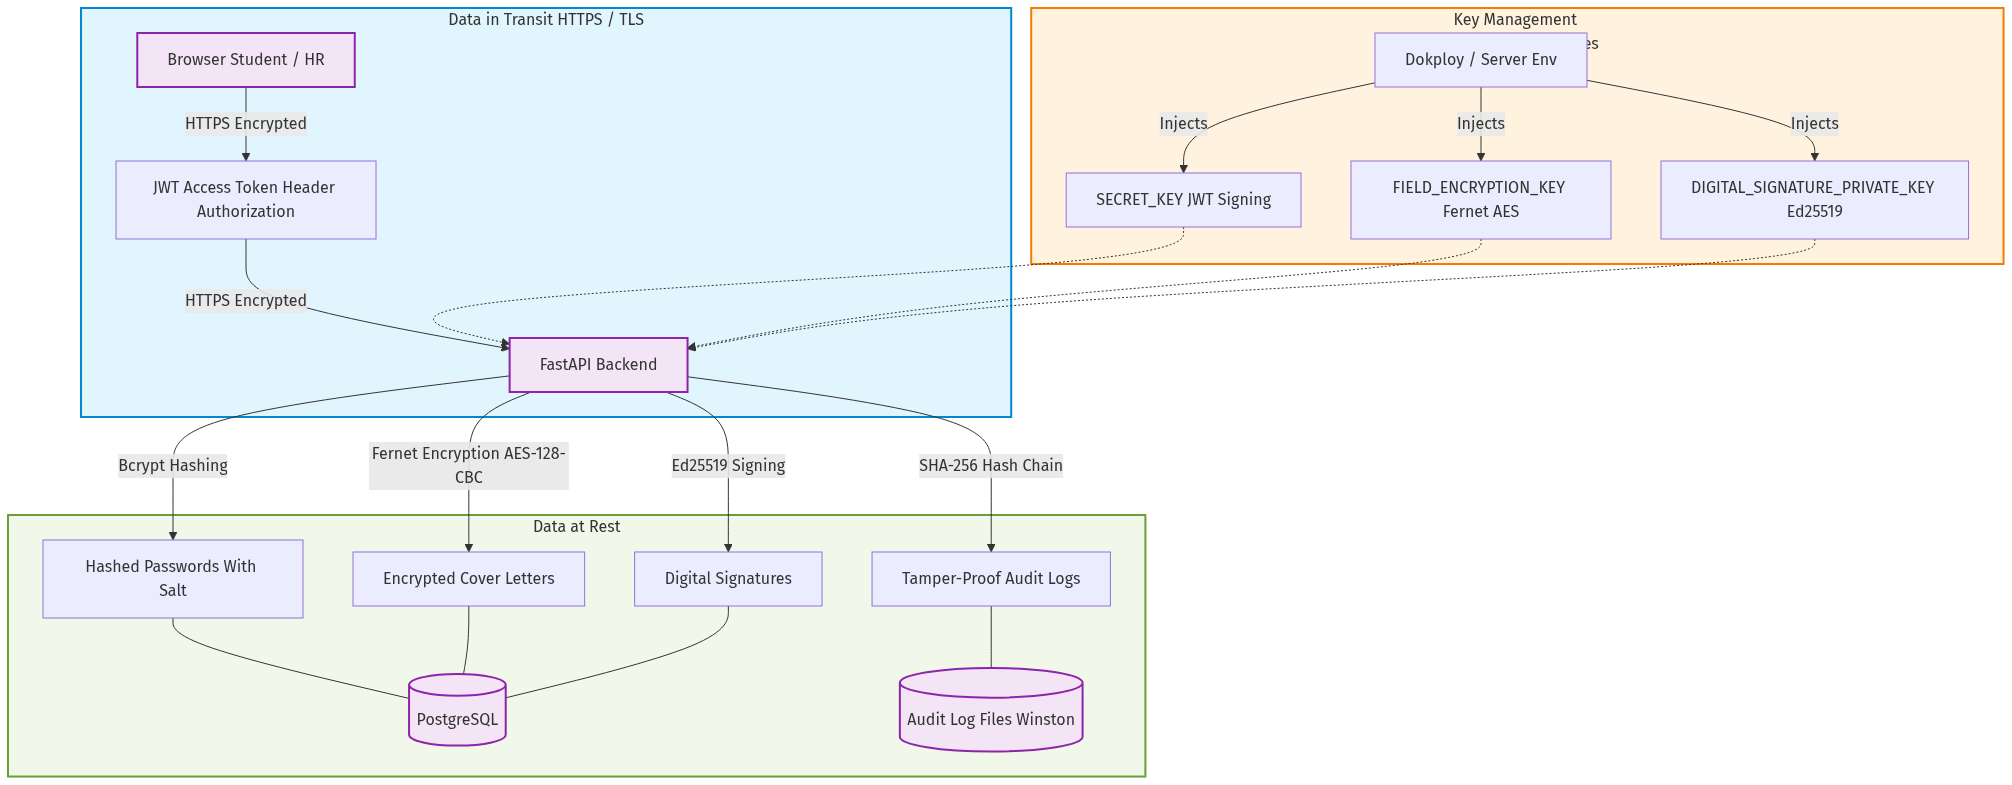
\includegraphics[width=0.92\textwidth]{images/security_architecture}
  \caption{Arsitektur keamanan TUMBUH: aliran data antarkomponen,
           penempatan kontrol kriptografi, dan skema manajemen kunci.}
  \label{fig:arsitektur}
\end{figure}

\subsection{Pemodelan Ancaman dan Pemetaan Kontrol}

Pemodelan ancaman dilakukan menggunakan kerangka STRIDE untuk
mengkategorikan ancaman secara sistematis. Enam kategori ancaman utama
beserta kontrol yang ditetapkan dirangkum dalam Tabel~\ref{tab:threatmap}.

\begin{table}[H]
  \caption{Pemetaan ancaman terhadap kontrol keamanan pada TUMBUH}
  \label{tab:threatmap}
  \centering
  \begin{tabularx}{\textwidth}{X X}
    \toprule
    Ancaman & Kontrol yang diterapkan \\
    \midrule
    Pencurian akun dan tebak paksa kata sandi
      & \textit{Password hashing} bcrypt, \textit{rate limiting},
        verifikasi surel \\
    Akses tidak sah ke data pengguna lain
      & RBAC, pemeriksaan kepemilikan, kontrol akses dokumen CV \\
    Kebocoran data sensitif dari basis data
      & Enkripsi tingkat kolom Fernet (AES-128-CBC + HMAC-SHA256) \\
    Manipulasi dan penyangkalan status lamaran
      & Tanda tangan digital Ed25519, jejak audit \\
    Pemalsuan atau penghapusan catatan audit
      & Rantai \textit{hash} SHA-256 (\textit{tamper evidence}) \\
    Kebocoran kunci kriptografi
      & Variabel lingkungan, tanpa \textit{hardcoded keys} \\
    \bottomrule
  \end{tabularx}
\end{table}

\subsection{Alat dan Bahan}

Tabel~\ref{tab:tools} merangkum komponen dan pustaka yang digunakan.
Pemilihan pustaka mengutamakan implementasi kriptografi yang sudah
diaudit komunitas, bukan implementasi mandiri.

\begin{table}[H]
  \caption{Komponen dan pustaka utama beserta fungsi keamanannya}
  \label{tab:tools}
  \centering
  \begin{tabularx}{\textwidth}{l l X}
    \toprule
    Komponen & Teknologi & Fungsi keamanan \\
    \midrule
    \textit{Frontend}    & React + Vite         & Penyimpanan token, permintaan terautentikasi \\
    \textit{Backend}     & FastAPI + SQLAlchemy & Logika AAA, validasi masukan, kriptografi \\
    Audit                & Express + Winston    & Pencatatan audit dan rantai \textit{hash} \\
    Basis data           & PostgreSQL           & Penyimpanan, \textit{parameterized query} \\
    \textit{Hashing}     & bcrypt 4.2.0         & \textit{Hashing} kata sandi dengan \textit{salt} \\
    Token                & python-jose 3.3.0    & Penerbitan dan verifikasi JWT (HS256) \\
    Kriptografi          & cryptography (PyCA)  & Enkripsi kolom (Fernet) dan tanda tangan (Ed25519) \\
    OAuth                & google-auth 2.45.0   & Verifikasi token identitas Google \\
    \textit{Rate limit}  & slowapi 0.1.9        & Pembatasan laju permintaan per IP \\
    \bottomrule
  \end{tabularx}
\end{table}

\subsection{Manajemen Kunci}

Tidak ada kunci kriptografi yang ditanamkan langsung dalam kode sumber.
Tiga rahasia utama dikelola melalui variabel lingkungan:
\texttt{SECRET\_KEY} untuk penandatanganan JWT,
\texttt{FIELD\_ENCRYPTION\_KEY} sebagai kunci simetris Fernet, dan
\texttt{DIGITAL\_SIGNATURE\_PRIVATE\_KEY} sebagai \textit{seed}
derivasi kunci Ed25519. Berkas konfigurasi yang memuat rahasia
dikecualikan dari repositori melalui \texttt{.gitignore}.

Pada lingkungan pengembangan, kunci Fernet dan \textit{seed} Ed25519
dapat diturunkan secara deterministik dari \texttt{SECRET\_KEY}
menggunakan SHA-256 untuk menyederhanakan konfigurasi awal, sedangkan
pada produksi setiap kunci disuntikkan secara eksplisit dan independen
\citep{NISTSP80057}. Pemisahan ini memastikan bocornya satu kunci tidak
otomatis mengompromikan kunci lainnya.

\subsection{Prosedur Pengujian}

Pengujian dilakukan menggunakan \texttt{pytest} terhadap basis data
SQLite \textit{in-memory} sehingga tidak bergantung pada infrastruktur
produksi. Sembilan skenario dirancang untuk memverifikasi tiga properti
keamanan utama: kerahasiaan (tiga skenario), integritas tanda tangan
(satu skenario), otorisasi (dua skenario), dan keamanan akun (tiga
skenario). Keluaran \texttt{pytest} diarsipkan di folder
\texttt{05\_Testing\_Logs} pada repositori.

\subsection{Prosedur Benchmark Kinerja}

Untuk memenuhi kebutuhan analisis kuantitatif, benchmark tambahan
dilakukan menggunakan skrip \texttt{benchmark\_security.py}. Benchmark
ini sengaja tidak mengakses basis data dan tidak melakukan panggilan
jaringan agar biaya yang terukur berfokus pada operasi keamanan inti:
bcrypt, JWT, Fernet, dan Ed25519. Baseline \textit{before} bersifat
sintetis, yaitu jalur login dengan perbandingan kata sandi plaintext,
jalur submit dengan surat lamaran plaintext, dan jalur read dengan
pembacaan plaintext. Baseline \textit{after} mengukur jalur aman:
login menggunakan verifikasi bcrypt dan penerbitan JWT, submit
menggunakan validasi JWT, enkripsi Fernet, dan penandatanganan
Ed25519, sedangkan read menggunakan validasi JWT dan dekripsi Fernet.

Benchmark dijalankan dengan 1000 iterasi untuk operasi cepat dan 10
iterasi untuk operasi bcrypt karena bcrypt memang dirancang lebih mahal
secara komputasi. Audit logging tidak dihitung dalam benchmark karena
backend mengirim event audit secara asinkron; yang diukur adalah biaya
kriptografi dan validasi token pada proses aplikasi utama.

Kode~\ref{lst:benchmark} memperlihatkan cuplikan inti skrip benchmark:
pengukuran durasi tiap operasi, jalur aman untuk login, submit, dan
read, serta perhitungan ukuran plaintext dan ciphertext. Ketiga jalur
aman tersebut kemudian dibandingkan terhadap baseline plaintext.

\begin{lstlisting}[language=Python,
  caption={Cuplikan benchmark untuk mengukur overhead login, submit,
           read, dan ukuran data terenkripsi},
  label={lst:benchmark}]
def time_operation(name: str, iterations: int, fn):
    durations = []
    for _ in range(iterations):
        start = time.perf_counter_ns()
        fn()
        elapsed_ms = (time.perf_counter_ns() - start) / 1_000_000
        durations.append(elapsed_ms)
    return {
        "name": name,
        "mean_ms": statistics.fmean(durations),
        "median_ms": statistics.median(durations),
        "p95_ms": percentile(durations, 0.95),
    }

def login_crypto_path():
    AuthService.verify_password(PASSWORD, password_hash)
    AuthService.create_access_token(token_data)
    AuthService.create_refresh_token(token_data)

def submit_crypto_path():
    AuthService.decode_token(access_token)
    security_service.encrypt_text(COVER_LETTER)
    security_service.sign_payload(signature_payload)

def read_crypto_path():
    AuthService.decode_token(access_token)
    security_service.decrypt_text(encrypted_letter)

raw_bytes = len(COVER_LETTER.encode("utf-8"))
encrypted_bytes = len((encrypted_letter or "").encode("utf-8"))
\end{lstlisting}

% =================================================================
\section{HASIL DAN PEMBAHASAN}
% =================================================================

\subsection{Autentikasi}

Autentikasi pada TUMBUH berjalan melalui tiga jalur yang saling
melengkapi. Jalur pertama berbasis surel dan kata sandi: saat
pendaftaran, sistem memvalidasi format surel, memeriksa domain
institusional (mahasiswa wajib menggunakan \texttt{@ipb.ac.id}),
memeriksa duplikasi, melakukan \textit{hashing} kata sandi, lalu
menerbitkan token verifikasi surel sekali pakai yang disimpan dalam
bentuk \textit{hash} SHA-256 dengan masa berlaku 24 jam. Saat masuk,
sistem memeriksa kecocokan kata sandi, status verifikasi surel, dan
status keaktifan akun sebelum token JWT diterbitkan. Pemisahan kondisi
ini disengaja agar akun yang belum diverifikasi atau sudah dinonaktifkan
tidak dapat memperoleh token yang valid.

Token diterbitkan menggunakan algoritma HS256, dengan \textit{access
token} berlaku 60 menit dan \textit{refresh token} berlaku tujuh hari.
Sistem secara eksplisit memverifikasi bahwa \textit{refresh token}
tidak dapat digunakan sebagai \textit{access token} untuk memanggil
\textit{endpoint} terlindungi. Untuk autentikasi melalui Google, token
identitas yang diterima diverifikasi tanda tangannya, audiensnya, dan
masa berlakunya sebelum identitas dipercaya \citep{RFC6749, RFC6819}.
Tidak ada kata sandi Google yang disimpan di sisi TUMBUH.

\subsection{Otorisasi}

Otorisasi diterapkan dalam dua lapisan. Lapisan pertama adalah
pembatasan berbasis peran dengan tiga peran yaitu \texttt{student},
\texttt{hr}, dan \texttt{admin}, diimplementasikan sebagai pabrik
dependensi \texttt{require\_role()} pada Kode~\ref{lst:rbac}. Fungsi
ini menolak permintaan dengan HTTP 403 jika peran tidak sesuai dan
dikaitkan ke \textit{endpoint} melalui \textit{dependency injection}
FastAPI, sehingga kontrol ini tidak bisa dilewati tanpa mengubah
definisi \textit{endpoint} itu sendiri.

\begin{lstlisting}[language=Python,
  caption={Pabrik dependensi RBAC yang menolak akses dengan HTTP 403
           bila peran tidak sesuai},
  label={lst:rbac}]
def require_role(required_role: str):
    def _check_role(
        current_user: User = Depends(get_current_user)
    ) -> User:
        if current_user.role.value != required_role:
            raise HTTPException(
                status_code=status.HTTP_403_FORBIDDEN,
                detail=f"Access denied. Required role: {required_role}",
            )
        return current_user
    return _check_role
\end{lstlisting}

Lapisan kedua adalah pemeriksaan kepemilikan. HR hanya dapat mengelola
pelamar dari perusahaannya sendiri, baik untuk pembaruan status
individual maupun massal. Dokumen CV disimpan di direktori privat dan
tidak pernah dilayani sebagai berkas statis, sehingga setiap akses
melewati lapisan autentikasi dan otorisasi. Lapisan ini penting karena
memiliki peran yang benar saja tidak cukup jika pengguna masih bisa
mengakses data orang lain yang kebetulan berbagi peran yang sama
\citep{Sandhu1996}.

\subsection{Akuntansi dan Audit Logging}

Pencatatan aktivitas dilakukan oleh mikroservis audit berbasis Express
dan Winston yang menerima peristiwa dari \textit{backend}. Pemanggilan
bersifat \textit{fire-and-forget} pada utas latar belakang sehingga
kegagalan layanan audit tidak memblokir respons API utama. Peristiwa
yang dicatat mencakup registrasi, masuk berhasil dan gagal, penyegaran
token, pengiriman dan pembaruan lamaran, pelanggaran \textit{rate
limit}, serta kesalahan tak tertangani.

Integritas catatan dijaga dengan rantai \textit{hash} SHA-256. Setiap
peristiwa baru di-\textit{hash} bersama \textit{hash} peristiwa
sebelumnya sebagaimana ditunjukkan pada Kode~\ref{lst:chain}.
Penghapusan atau modifikasi satu entri akan memutus rantai dan dapat
dideteksi oleh fungsi verifikasi yang membaca \textit{log} secara
kronologis.

\begin{lstlisting}[language=Java,
  caption={Perantaian hash SHA-256 pada tiap entri audit;
           modifikasi satu entri memutus rantai},
  label={lst:chain}]
function chainAuditEvent(event) {
  const previousHash = loadLastHash(); // 'GENESIS' jika pertama
  const eventHash = crypto
    .createHash('sha256')
    .update(previousHash + ':' + canonicalJson(event))
    .digest('hex');
  return {
    ...event,
    previousHash,
    eventHash,
    integrityAlgorithm: 'SHA-256 hash chain',
  };
}
\end{lstlisting}

\subsection{Hashing Kata Sandi}

Kata sandi tidak pernah disimpan dalam bentuk aslinya. bcrypt dipilih
karena dua sifatnya yang saling melengkapi: \textit{salt} otomatis per
kata sandi yang mencegah serangan \textit{rainbow table}, dan faktor
biaya yang dapat disesuaikan \citep{Provos1999}. Pada faktor biaya 12
yang digunakan, setiap operasi \textit{hashing} membutuhkan waktu
sekitar 200--300 ms pada \textit{hardware} umum, cukup menyulitkan
serangan tebak paksa berskala besar tanpa terasa mengganggu pengguna.
Faktor ini pun dapat dinaikkan di masa depan tanpa mengubah kode.
Implementasinya ditunjukkan pada Kode~\ref{lst:bcrypt}. \textit{Field}
\texttt{hashed\_password} tidak dideklarasikan dalam skema respons API
sehingga tidak mungkin bocor melalui \textit{endpoint} manapun.

\begin{lstlisting}[language=Python,
  caption={Operasi hashing dan verifikasi kata sandi menggunakan
           bcrypt dengan salt otomatis},
  label={lst:bcrypt}]
@staticmethod
def hash_password(password: str) -> str:
    return _bcrypt.hashpw(
        password.encode("utf-8"), _bcrypt.gensalt()
    ).decode("utf-8")

@staticmethod
def verify_password(plain: str, hashed: str) -> bool:
    return _bcrypt.checkpw(
        plain.encode("utf-8"), hashed.encode("utf-8")
    )
\end{lstlisting}

\subsection{Enkripsi Tingkat Kolom}

Surat lamaran dienkripsi sebelum disimpan ke basis data menggunakan
Fernet, yang menggabungkan AES-128-CBC dengan HMAC-SHA256 untuk
memberikan enkripsi terautentikasi \citep{NIST2001, Katz2014}. Modifikasi
sekecil apapun pada \textit{ciphertext} menyebabkan dekripsi gagal
karena HMAC akan tidak cocok. Enkripsi tingkat kolom dipilih atas
enkripsi penuh basis data karena granularitasnya; hanya kolom yang
memerlukan perlindungan ekstra yang dienkripsi, sementara kolom lain
tetap bisa dicari dan diindeks secara efisien.

Kode~\ref{lst:fernet} menunjukkan fungsi enkripsi dan dekripsi. Nilai
terenkripsi diberi awalan \texttt{enc:v1:} untuk menandai status
enkripsi, mencegah enkripsi ganda, dan menyediakan jalur migrasi jika
algoritma diganti. Di basis data, surat lamaran tersimpan sebagai
\textit{ciphertext}; di respons API, nilai dikembalikan setelah
didekripsi. Kebocoran basis data tidak serta-merta mengungkap isi surat
lamaran karena penyerang tetap memerlukan kunci enkripsi yang disimpan
terpisah di luar basis data \citep{Cryptography2024}.

\begin{lstlisting}[language=Python,
  caption={Enkripsi tingkat kolom Fernet dengan awalan versi
           untuk migrasi algoritma yang aman},
  label={lst:fernet}]
ENCRYPTED_PREFIX = "enc:v1:"

def encrypt_text(self, value: str | None) -> str | None:
    if value is None or value.startswith(ENCRYPTED_PREFIX):
        return value
    token = self._fernet.encrypt(
        value.encode("utf-8")
    ).decode("utf-8")
    return f"{ENCRYPTED_PREFIX}{token}"

def decrypt_text(self, value: str | None) -> str | None:
    if value is None or not value.startswith(ENCRYPTED_PREFIX):
        return value
    raw = value.removeprefix(ENCRYPTED_PREFIX).encode("utf-8")
    try:
        return self._fernet.decrypt(raw).decode("utf-8")
    except InvalidToken:
        return "[encrypted value could not be decrypted]"
\end{lstlisting}

\subsection{Tanda Tangan Digital}

Setiap peristiwa kritis dalam siklus lamaran, yaitu pengiriman oleh
mahasiswa dan perubahan status oleh HR, ditandatangani menggunakan
Ed25519. Sebelum ditandatangani, \textit{payload} dikanonikalisasi
menjadi JSON dengan kunci terurut agar deterministik. \textit{Payload},
tanda tangan, dan nama algoritma disimpan bersama catatan lamaran di
basis data. Kode~\ref{lst:sign} menunjukkan fungsi penandatanganan dan
verifikasi.

\begin{lstlisting}[language=Python,
  caption={Penandatanganan payload kanonik dan verifikasi tanda
           tangan Ed25519 untuk jaminan non-repudiasi},
  label={lst:sign}]
def sign_payload(self, payload: dict) -> str:
    canonical = self._canonical_json(payload).encode("utf-8")
    signature = self._private_key.sign(canonical)
    return base64.urlsafe_b64encode(signature).decode("ascii")

def verify_signature(
    self, payload: dict, signature: str
) -> bool:
    try:
        raw = base64.urlsafe_b64decode(
            signature.encode("ascii")
        )
        self._public_key.verify(
            raw,
            self._canonical_json(payload).encode("utf-8")
        )
        return True
    except Exception:
        return False
\end{lstlisting}

\textit{Endpoint} verifikasi yang hanya bisa diakses admin memungkinkan
pemeriksaan keaslian tanda tangan kapan saja. Jika \textit{payload}
lamaran pernah dimodifikasi setelah penandatanganan, verifikasi akan
gagal. Mahasiswa tidak dapat menyangkal pengiriman lamaran dan HR tidak
dapat menyangkal perubahan status karena klaim tersebut dapat dibantah
secara kriptografis \citep{Bernstein2012, RFC8032}.

\subsection{Kontrol Keamanan Pendukung}

Sejumlah kontrol pelengkap diterapkan mengikuti prinsip
\textit{defense in depth} \citep{Anderson2020}. \textit{Security
headers} \texttt{X-Content-Type-Options}, \texttt{X-Frame-Options},
dan \texttt{Referrer-Policy} ditambahkan pada setiap respons untuk
memitigasi \textit{MIME sniffing} dan \textit{clickjacking}.
\textit{Rate limiting} berbasis IP membatasi 5 hingga 10 permintaan
per menit pada \textit{endpoint} autentikasi. CORS dikonfigurasi
dengan daftar \textit{origin} yang diizinkan secara eksplisit.
Unggahan berkas divalidasi berdasarkan tipe MIME dan ukuran, dengan
nama berkas yang dibangkitkan ulang. Verifikasi surel menggunakan
token sekali pakai berbasis SHA-256 yang kedaluwarsa setelah 24 jam.
Pencegahan injeksi SQL diperoleh melalui \textit{parameterized query}
pada ORM SQLAlchemy, dan validasi masukan dijamin oleh skema Pydantic
di setiap \textit{endpoint} \citep{OWASP2021}.

\subsection{Integrasi pada Alur Utama Aplikasi}

Semua modul kriptografi tertanam langsung pada alur bisnis utama
aplikasi. Kode~\ref{lst:workflow} menunjukkan \textit{endpoint}
pengiriman lamaran, tempat lima lapis keamanan berjalan dalam satu
transaksi yang berurutan.

\begin{lstlisting}[language=Python,
  caption={Alur pengiriman lamaran: validasi token dan peran,
           enkripsi kolom, tanda tangan digital, audit logging,
           dan dekripsi untuk respons},
  label={lst:workflow}]
@router.post("/applications")
async def submit_application(
    data: ApplicationCreate,
    background_tasks: BackgroundTasks,
    user: User = Depends(require_role("student")),
    db: Session = Depends(get_db),
):
    # 1. Enkripsi sebelum penyimpanan ke basis data
    encrypted = security.encrypt_text(data.application_letter)
    app = Application(
        student_id=user.id, job_id=data.job_id,
        application_letter=encrypted,
    )
    db.add(app); db.flush()

    # 2. Tanda tangan digital untuk non-repudiasi
    payload = {
        "action": "SUBMIT", "student_id": user.id,
        "job_id": data.job_id, "application_id": app.id,
        "timestamp": datetime.utcnow().isoformat(),
    }
    app.signature = security.sign_payload(payload)
    app.signature_payload = json.dumps(payload, sort_keys=True)
    app.signature_algorithm = "Ed25519"
    db.commit()

    # 3. Audit logging di latar belakang (fire-and-forget)
    background_tasks.add_task(
        audit.log_event, "APPLICATION_SUBMITTED", payload
    )

    # 4. Respons dengan nilai terdekripsi
    return ApplicationResponse(
        id=app.id,
        application_letter=security.decrypt_text(encrypted),
    )
\end{lstlisting}

Urutan operasi ini bukan sekadar pilihan gaya. Enkripsi harus terjadi
sebelum penyimpanan ke basis data; penandatanganan harus terjadi setelah
\texttt{flush()} agar \texttt{application.id} sudah tersedia dalam
\textit{payload}; dan \textit{audit logging} dijalankan di latar
belakang agar kegagalannya tidak membatalkan transaksi utama.

\subsection{Perbandingan Fitur Keamanan}

Tabel~\ref{tab:compare} membandingkan fitur keamanan TUMBUH dengan dua
profil implementasi yang umum dijumpai.

\begin{table}[H]
  \caption{Perbandingan fitur keamanan TUMBUH dengan profil implementasi
           yang umum}
  \label{tab:compare}
  \centering
  \begin{tabularx}{\textwidth}{X c c c}
    \toprule
    Fitur keamanan
      & \makecell{Sistem akademik\\konvensional}
      & \makecell{Aplikasi web\\umum}
      & TUMBUH \\
    \midrule
    \textit{Password hashing} adaptif   & Sebagian & \checkmark & \checkmark \\
    Token JWT \textit{stateless}        & $\times$ & \checkmark & \checkmark \\
    OAuth identitas pihak ketiga        & $\times$ & Sebagian   & \checkmark \\
    RBAC dengan \textit{ownership check}& $\times$ & Sebagian   & \checkmark \\
    Enkripsi tingkat kolom              & $\times$ & $\times$   & \checkmark \\
    Tanda tangan digital per peristiwa  & $\times$ & $\times$   & \checkmark \\
    Audit \textit{log} berrantai hash   & $\times$ & $\times$   & \checkmark \\
    Manajemen kunci via variabel lingkungan & $\times$ & Sebagian & \checkmark \\
    \bottomrule
  \end{tabularx}
\end{table}

\noindent
($\checkmark$ = diterapkan; $\times$ = tidak ada; Sebagian = diterapkan
dengan variasi kualitas)

Enkripsi tingkat kolom dan tanda tangan digital per peristiwa adalah
dua fitur yang paling membedakan pendekatan TUMBUH dari implementasi
konvensional. Keduanya menjawab langsung dua ancaman yang paling sulit
ditangani: kebocoran basis data dan penyangkalan tindakan.

\subsection{Hasil Pengujian}

Tabel~\ref{tab:uji} merangkum hasil pengujian unit. Seluruh sembilan
skenario berhasil dalam satu kali eksekusi \texttt{pytest}.

\begin{table}[H]
  \caption{Ringkasan hasil pengujian unit terhadap sembilan skenario
           keamanan}
  \label{tab:uji}
  \centering
  \begin{tabularx}{\textwidth}{X l}
    \toprule
    Skenario pengujian & Hasil \\
    \midrule
    \textit{Roundtrip} enkripsi-dekripsi surat lamaran           & Lulus \\
    Deteksi pemalsuan tanda tangan digital                       & Lulus \\
    Penonaktifan akun memblokir proses masuk berikutnya          & Lulus \\
    Penghapusan akun mensyaratkan kecocokan surel                & Lulus \\
    Penggantian kata sandi via \textit{reset} surel              & Lulus \\
    Pengguna \texttt{student} ditolak pada sumber daya admin     & Lulus \\
    Pengguna \texttt{admin} diizinkan pada sumber daya admin     & Lulus \\
    Data terenkripsi tidak terbaca sebagai teks biasa            & Lulus \\
    \textit{Ciphertext} yang dirusak ditolak saat dekripsi       & Lulus \\
    \midrule
    \textbf{Total} & \textbf{9/9} \\
    \bottomrule
  \end{tabularx}
\end{table}

Skenario ketiga mengonfirmasi bahwa kondisi keaktifan akun diperiksa
sebagai bagian dari autentikasi, tidak hanya saat akun dibuat. Skenario
kedelapan dan kesembilan bersama-sama membuktikan properti enkripsi
terautentikasi Fernet bekerja sesuai desain; data hanya terbaca dalam
kondisi normal dan modifikasi sekecil apapun pada \textit{ciphertext}
menyebabkan penolakan. Skenario keenam dan ketujuh mengonfirmasi RBAC
bekerja secara simetris untuk menolak dan mengizinkan akses secara
tepat.

\subsection{Analisis Kinerja Kontrol Keamanan}

Tabel~\ref{tab:perf} menunjukkan hasil benchmark before-vs-after untuk
tiga jalur yang paling relevan terhadap kontrol keamanan: login, submit
lamaran, dan read lamaran. Angka \textit{before} bukan berasal dari
versi lama aplikasi, melainkan baseline sintetis untuk menunjukkan
biaya tambahan dari operasi keamanan. Dengan demikian, tabel ini
menjelaskan trade-off performa dari kontrol yang ditambahkan, bukan
membandingkan dua rilis aplikasi yang berbeda.

\begin{table}[H]
  \caption{Benchmark before-vs-after operasi keamanan TUMBUH}
  \label{tab:perf}
  \centering
  \begin{tabularx}{\textwidth}{X r r r}
    \toprule
    Use case & Before mean (ms) & After mean (ms) & Delta (ms) \\
    \midrule
    Login path  & 0,0002 & 276,4189 & 276,4187 \\
    Submit path & 0,0002 & 0,1224   & 0,1222 \\
    Read path   & 0,0001 & 0,0625   & 0,0624 \\
    \bottomrule
  \end{tabularx}
\end{table}

Overhead terbesar berada pada jalur login. Pada benchmark komponen,
verifikasi bcrypt membutuhkan rata-rata 273,085 ms. Biaya ini bukan
efek samping yang tidak diinginkan, melainkan karakteristik desain
bcrypt: proses hashing dan verifikasi dibuat mahal agar serangan tebak
paksa menjadi lebih sulit dilakukan dalam skala besar. Karena login
tidak terjadi sesering operasi baca data, overhead ratusan milidetik
masih dapat diterima untuk cakupan proyek ini, terutama jika digabungkan
dengan pembatasan laju permintaan pada endpoint autentikasi.

Sebaliknya, overhead jalur submit dan read relatif kecil. Submit path
membutuhkan rata-rata 0,1224 ms setelah kontrol keamanan, yang mencakup
validasi JWT, enkripsi Fernet terhadap surat lamaran, dan tanda tangan
digital Ed25519. Read path membutuhkan rata-rata 0,0625 ms karena hanya
melakukan validasi JWT dan dekripsi Fernet. Hasil ini menunjukkan bahwa
bottleneck keamanan utama berada pada bcrypt, bukan pada enkripsi kolom
atau tanda tangan digital.

\begin{table}[H]
  \caption{Rincian waktu operasi keamanan pada benchmark lokal}
  \label{tab:perfdetail}
  \centering
  \begin{tabularx}{\textwidth}{X r r r}
    \toprule
    Operasi & Mean (ms) & Median (ms) & P95 (ms) \\
    \midrule
    bcrypt verify & 273,085 & 272,612 & 277,061 \\
    JWT encode access+refresh & 0,037 & 0,033 & 0,055 \\
    JWT decode access & 0,034 & 0,033 & 0,045 \\
    Fernet encrypt cover letter & 0,021 & 0,020 & 0,028 \\
    Fernet decrypt cover letter & 0,019 & 0,018 & 0,024 \\
    Ed25519 sign payload & 0,041 & 0,040 & 0,046 \\
    Ed25519 verify payload & 0,123 & 0,122 & 0,128 \\
    \bottomrule
  \end{tabularx}
\end{table}

\subsection{Overhead Ukuran Data Terenkripsi}

Selain waktu eksekusi, enkripsi tingkat kolom juga menambah ukuran data
yang disimpan. Pada sampel surat lamaran berukuran 1007 byte, format
terenkripsi dengan awalan \texttt{enc:v1:} menghasilkan nilai tersimpan
sebesar 1427 byte. Hasil ini dirangkum pada Tabel~\ref{tab:sizeoverhead}.

\begin{table}[H]
  \caption{Overhead ukuran data setelah enkripsi surat lamaran}
  \label{tab:sizeoverhead}
  \centering
  \begin{tabularx}{\textwidth}{X r r r}
    \toprule
    Field & Plaintext (byte) & Encrypted (byte) & Overhead \\
    \midrule
    Cover letter & 1007 & 1427 & 420 byte / 1,42x \\
    \bottomrule
  \end{tabularx}
\end{table}

Kenaikan ukuran ini berasal dari metadata Fernet, seperti timestamp,
initialization vector, HMAC, dan encoding base64. Untuk field teks
pendek seperti surat lamaran, overhead 1,42x masih wajar. Namun jika
enkripsi diperluas ke file besar seperti CV, strategi yang lebih tepat
adalah enkripsi file atau envelope encryption dengan manajemen kunci
yang lebih matang.

Pengujian ini terbatas pada \textit{unit testing} dengan basis data
\textit{in-memory}. Beberapa vektor serangan seperti \textit{timing
attacks}, keamanan konfigurasi TLS di produksi, dan kerentanan di
\textit{frontend} belum tercakup dan memerlukan \textit{integration
testing} serta \textit{penetration testing} untuk penilaian yang lebih
menyeluruh.

% =================================================================
\section{SIMPULAN}
% =================================================================

Penelitian ini berhasil mengimplementasikan kerangka keamanan berlapis
pada TUMBUH yang mengintegrasikan protokol AAA, enkripsi tingkat kolom
Fernet, tanda tangan digital Ed25519, dan rantai \textit{hash} SHA-256
dalam satu alur kerja yang kohesif. Autentikasi diterapkan melalui
bcrypt, JWT HS256, dan Google OAuth; otorisasi melalui RBAC tiga peran
yang dilengkapi pemeriksaan kepemilikan; dan akuntansi melalui
mikroservis audit dengan rantai \textit{hash} SHA-256. Kebocoran basis
data tidak serta-merta mengungkap surat lamaran karena kolom tersebut
dienkripsi, sedangkan penyangkalan peristiwa lamaran dapat dibantah
dengan tanda tangan Ed25519 yang tersimpan bersama setiap catatan.
Seluruh kunci dikelola melalui variabel lingkungan. Pengujian unit
terhadap sembilan skenario menghasilkan sembilan kelulusan, membuktikan
kontrol yang diimplementasikan memenuhi sasaran kerahasiaan, integritas,
dan akuntabilitas dalam cakupan yang diuji. Analisis kinerja
menunjukkan bahwa biaya terbesar berada pada login karena verifikasi
bcrypt, yaitu 276,4189 ms, sedangkan overhead submit dan read tetap
di bawah 1 ms, masing-masing 0,1224 ms dan 0,0625 ms. Enkripsi surat
lamaran menambah ukuran data dari 1007 byte menjadi 1427 byte atau
1,42x. Dengan demikian, kontrol keamanan utama memberikan peningkatan
perlindungan yang signifikan dengan overhead yang terukur dan masih
dapat diterima pada cakupan proyek ini. Untuk pengembangan selanjutnya,
rotasi kunci berkala melalui mekanisme awalan versi, perluasan
enkripsi ke atribut sensitif lain, autentikasi dua faktor, serta
\textit{integration testing}, \textit{load testing}, dan
\textit{penetration testing} menjadi prioritas yang direkomendasikan.

% =================================================================
\section*{UCAPAN TERIMA KASIH}
% =================================================================

Penulis menyampaikan terima kasih kepada Dr.\,Shelvie Nidya Neyman dan
Endang P.\,Giri, S.Kom, M.Kom selaku dosen mata kuliah Keamanan
Informasi (KOM1315) IPB University atas bimbingan selama pelaksanaan
proyek ini.

% =================================================================
\bibliographystyle{ipb}
\bibliography{refs/daftar_pustaka}
% =================================================================

\end{document}
